\documentclass[10pt,letterpaper]{article}
\usepackage[margin=0.5in]{geometry}
\usepackage{enumitem}
\usepackage{booktabs}
\usepackage{hyperref}
\usepackage{xcolor}
\usepackage{tikz}
\usetikzlibrary{shapes.geometric,arrows.meta,positioning,fit,backgrounds,calc,shadows}
\usepackage{titlesec}
\usepackage{microtype}

\definecolor{awsblue}{RGB}{35, 47, 62}
\definecolor{awsorange}{RGB}{255, 153, 0}
\definecolor{cloudbg}{RGB}{248, 250, 253}
\definecolor{vpcbg}{RGB}{239, 246, 252}
\definecolor{boxborder}{RGB}{180, 195, 210}
\definecolor{customemerald}{RGB}{38, 130, 60}

\titleformat{\section}{\large\bfseries}{}{0em}{}[\vspace{-4pt}\rule{\textwidth}{0.4pt}\vspace{-4pt}]
\titleformat{\subsection}{\normalsize\bfseries}{}{0em}{}
\titlespacing*{\section}{0pt}{4pt}{2pt}
\titlespacing*{\subsection}{0pt}{3pt}{1pt}
\setlist{nosep,leftmargin=1.2em}

\begin{document}
\pagestyle{empty}

\begin{center}
{\Large\textbf{Nimbus P4: Foundation and Cloud Infrastructure Summary}}\\[2pt]
{\small\textbf{Live Deployment:} AWS Account \texttt{930124786284}, Region \texttt{ap-south-1}, Service: \texttt{nimbus-ds252-service}}
\end{center}
\vspace{-6pt}

\section{Executive Overview of P4 Deliverables}
Person 4 delivered the production cloud infrastructure and deployment foundation for Project Nimbus, transitioning the system from local simulation to a live, monitored AWS environment. The implementation strictly adheres to a vanilla, lightweight stack: standard library Python HTTP server (\texttt{server.py}), standard AWS SDK (\texttt{boto3}), and vanilla browser assets (HTML, CSS, JavaScript) without external application frameworks.

\begin{itemize}
  \item \textbf{Live Cloud Service:} Automated Terraform provisioning and containerized deployment on AWS ECS Fargate, served via Amazon API Gateway HTTP API (\texttt{qrgdidp9te.execute-api.ap-south-1.amazonaws.com}).
  \item \textbf{Requester Web Application:} Lightweight hospital logistics portal (\texttt{static/requester.html}, \texttt{static/requester.js}) at root route (\texttt{/}) providing natural language item dispatch, clarification response intake, and real-time task status polling.
  \item \textbf{Operator Command Console:} Operational command dashboard (\texttt{static/operator.html}, \texttt{static/operator.js}) at \texttt{/operator} featuring live fleet telemetry, link fault monitoring, active task tracking, and runtime controls.
  \item \textbf{Operator Inventory Controls:} Direct inventory counters (\texttt{data/inventory.json}, \texttt{/inventory}) in the console with exactly two buttons: ``Set stock'' and ``Reset stock''. When tasks are leased, stock is automatically decremented. Memory can also be reset via \texttt{POST /reset-memory}.
  \item \textbf{Active Pack Switch to \texttt{hospital\_sim6}:} Migrated the default domain configuration to \texttt{packs/hospital\_sim6} (ID: \texttt{hospital\_sim6@0.1.0:88d32afe}) across \texttt{packs/DEFAULT}, \texttt{Dockerfile}, and ECS task definition. This configures the six-robot Gazebo world (\texttt{R1}--\texttt{R3} in \texttt{east-wing}, \texttt{R4}--\texttt{R6} in \texttt{west-wing}) with P1 Gazebo map topology.
\end{itemize}

\section{Requester Application and Cloud Processing Path}

\subsection{Input Schema (\texttt{POST /requests})}
Hospital requests are submitted as JSON payloads to \texttt{POST /requests}:
\begin{itemize}
  \item \texttt{text} (\texttt{string}, required): Natural language request, e.g., \texttt{"Deliver a wheelchair to ward 3, routine."} or \texttt{"Need an infusion pump at 2B-12, urgent."}
  \item \texttt{message\_id} (\texttt{string}, required): Unique client UUID/token used for strict idempotency deduplication (PRD FR-8).
\end{itemize}

\subsection{Request Processing Pipeline}
\begin{enumerate}
  \item \textbf{Deduplication (\texttt{server.py:510}):} Incoming \texttt{message\_id} is evaluated under thread lock \texttt{\_STATE\_LOCK}. If previously recorded in store, the call immediately returns HTTP 200 with \texttt{\{"duplicate": true\}} without re-execution.
  \item \textbf{Context Assembly (\texttt{cloud/orchestrator.py:207}):} Orchestrator calls \texttt{build\_context()} to synthesize map topology nodes, active closures, fleet positions, battery states, stock counts, and prior task history.
  \item \textbf{Intent Parsing (\texttt{cloud/agent.py}, \texttt{cloud/llm.py}):} In \texttt{C1} mode, requests invoke Amazon Bedrock (\texttt{BedrockLLM}) with Nova-Lite to produce structured tool calls (\texttt{submit\_task\_spec} or \texttt{ask\_clarification}). If Bedrock is down or unreachable, the circuit breaker instantly diverts execution to the deterministic fallback (\texttt{RuleBasedLLM}) with reduced autonomy notification.
  \item \textbf{Domain Rule and Policy Check (\texttt{cloud/policy.py}, \texttt{cloud/allocator.py}):} Validates item constraints (e.g., paediatric equipment requirements under \texttt{SOP-PAED-01}), area closures, and isolation ward restrictions (\texttt{SOP-ISO-02}).
  \item \textbf{Cluster Allocation \& Routing (\texttt{cloud/allocator.py}):} Identifies candidate robot clusters (\texttt{east-wing} vs. \texttt{west-wing}), verifies equipment stock, computes shortest path on the Gazebo topology graph, and selects available robots.
  \item \textbf{Lease Synthesis (\texttt{cloud/leasebuilder.py}):} Constructs an authority lease with strict monotonic versioning, allowed/forbidden zones, robot sequences (\texttt{go\_to}, \texttt{wait}, \texttt{photo}, \texttt{report}), speed limits, and escalation triggers.
  \item \textbf{Inventory Decrement and State Persistence (\texttt{server.py:804}, \texttt{cloud/aws\_dynamo.py}):} Decrements local/persisted stock for the requested item and writes tasks, leases, and decision rows to DynamoDB tables.
\end{enumerate}

\subsection{Output Schema}
\begin{itemize}
  \item \textbf{Synchronous API Response (\texttt{POST /requests}):} Returns HTTP 201 Created:
  \begin{itemize}
    \item \texttt{\{"duplicate": false, "task\_id": "task-XXXXXX", "status": "leased" | "needs\_clarification", ...\}}
  \end{itemize}
  \item \textbf{Authority Lease Contract (\texttt{contracts/lease.schema.json}):} If leased, the authoritative contract provides:
  \begin{itemize}
    \item \texttt{lease\_id} (\texttt{string}): Globally unique identifier (e.g., \texttt{"lease-task-000027-v1"}).
    \item \texttt{version} (\texttt{integer}): Monotonic version number; newer versions completely supersede older versions.
    \item \texttt{priority} (\texttt{"routine"} or \texttt{"urgent"}): Task priority class.
    \item \texttt{deadline\_ts} and \texttt{expiry\_ts} (\texttt{ISO-8601}): Task deadline and hard expiry timestamps.
    \item \texttt{allowed\_zones} and \texttt{forbidden\_zones} (\texttt{array[string]}): Geofenced graph nodes.
    \item \texttt{speed\_limit} (\texttt{number}): Maximum speed limit in meters per second (1.0 m/s in simulation).
    \item \texttt{assigned\_robots} (\texttt{array[string]}): Designated robots from the pack fleet (e.g., \texttt{["R6"]}).
    \item \texttt{task\_sequence} (\texttt{array[object]}): Sequential robot commands with parameters and target nodes.
    \item \texttt{cluster\_id} (\texttt{"east-wing"} or \texttt{"west-wing"}): Assigned responsible edge cluster.
    \item \texttt{when\_to\_escalate} (\texttt{array[string]}): Guard conditions trigger escalation (e.g., \texttt{"door\_closed"}).
  \end{itemize}
\end{itemize}

\pagebreak
\section{Live AWS Infrastructure Architecture}
The cloud infrastructure is provisioned through modular Terraform configurations located in \texttt{infra/terraform/} and operates in AWS Account \texttt{930124786284}, Region \texttt{ap-south-1}.

\begin{center}
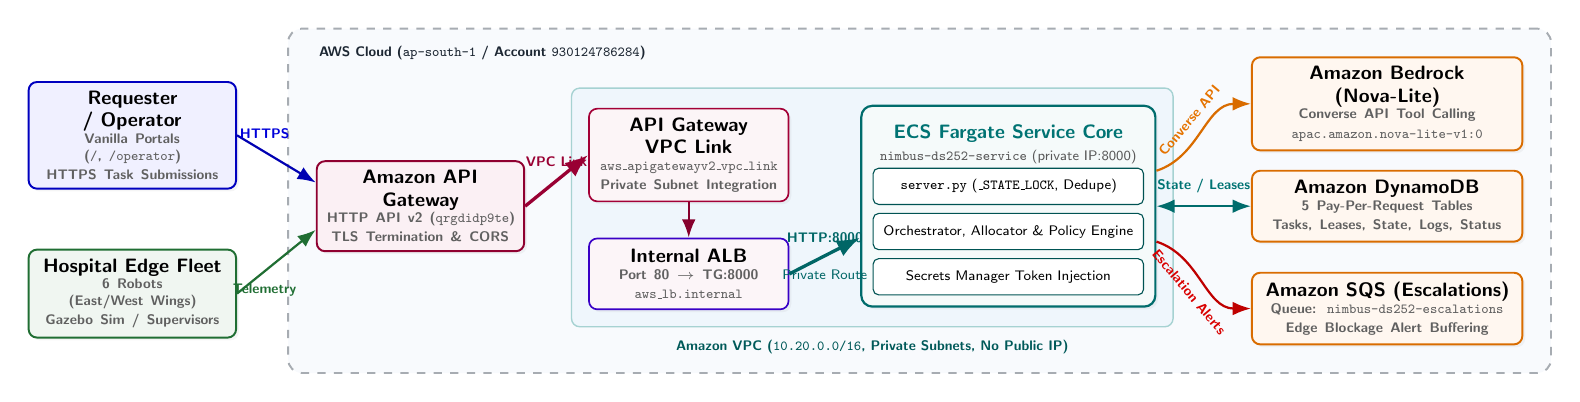
\begin{tikzpicture}[
  >=Latex,
  font=\sffamily,
  client/.style={
    draw=blue!75!black, fill=blue!6, rounded corners=3pt,
    text width=2.4cm, minimum height=1.05cm, align=center,
    font=\sffamily\scriptsize\bfseries, line width=0.7pt, drop shadow={opacity=0.08, shadow xshift=1pt, shadow yshift=-1pt}
  },
  gw/.style={
    draw=purple!75!black, fill=purple!6, rounded corners=3pt,
    text width=2.4cm, minimum height=1.05cm, align=center,
    font=\sffamily\scriptsize\bfseries, line width=0.7pt, drop shadow={opacity=0.08, shadow xshift=1pt, shadow yshift=-1pt}
  },
  privnet/.style={
    draw=purple!85!black, fill=purple!4, rounded corners=3pt,
    text width=2.3cm, minimum height=0.9cm, align=center,
    font=\sffamily\scriptsize\bfseries, line width=0.6pt, drop shadow={opacity=0.08, shadow xshift=1pt, shadow yshift=-1pt}
  },
  alb/.style={
    draw=blue!70!purple, fill=blue!4!purple!4, rounded corners=3pt,
    text width=2.3cm, minimum height=0.9cm, align=center,
    font=\sffamily\scriptsize\bfseries, line width=0.6pt, drop shadow={opacity=0.08, shadow xshift=1pt, shadow yshift=-1pt}
  },
  ecs/.style={
    draw=teal!85!black, fill=teal!4, rounded corners=4pt,
    text width=3.5cm, minimum height=2.55cm, align=center,
    font=\sffamily\scriptsize\bfseries, line width=0.8pt, drop shadow={opacity=0.08, shadow xshift=1pt, shadow yshift=-1pt}
  },
  subnode/.style={
    draw=teal!65!black, fill=white, rounded corners=2pt,
    text width=3.2cm, minimum height=0.46cm, align=center,
    font=\sffamily\tiny, line width=0.4pt
  },
  backend/.style={
    draw=orange!85!black, fill=orange!6, rounded corners=3pt,
    text width=3.2cm, minimum height=0.9cm, align=center,
    font=\sffamily\scriptsize\bfseries, line width=0.7pt, drop shadow={opacity=0.08, shadow xshift=1pt, shadow yshift=-1pt}
  },
  edge/.style={
    draw=customemerald!85!black, fill=customemerald!7, rounded corners=3pt,
    text width=2.4cm, minimum height=1.05cm, align=center,
    font=\sffamily\scriptsize\bfseries, line width=0.7pt, drop shadow={opacity=0.08, shadow xshift=1pt, shadow yshift=-1pt}
  }
]

  % Clients (Left)
  \node[client] (client) {Requester / Operator\\{\tiny\color{gray!75!black}Vanilla Portals (\texttt{/}, \texttt{/operator})\\[-1pt]HTTPS Task Submissions}};
  \node[edge, below=0.75cm of client] (fleet) {Hospital Edge Fleet\\{\tiny\color{gray!75!black}6 Robots (East/West Wings)\\[-1pt]Gazebo Sim / Supervisors}};

  % Ingress (API Gateway)
  \node[gw, right=1.0cm of client, yshift=-0.9cm] (apigw) {Amazon API Gateway\\{\tiny\color{gray!75!black}HTTP API v2 (\texttt{qrgdidp9te})\\[-1pt]TLS Termination \& CORS}};

  % Private Network Integration (VPC Link + Internal ALB)
  \node[privnet, right=0.8cm of apigw, yshift=0.65cm] (vpclink) {API Gateway VPC Link\\{\tiny\color{gray!75!black}\texttt{aws\_apigatewayv2\_vpc\_link}\\[-1pt]Private Subnet Integration}};
  \node[alb, below=0.45cm of vpclink] (alb) {Internal ALB\\{\tiny\color{gray!75!black}Port 80 $\rightarrow$ TG:8000\\[-1pt]\texttt{aws\_lb.internal}}};

  % ECS Compute Core (Middle)
  \node[ecs, right=0.9cm of vpclink, yshift=-0.65cm] (ecs) {};
  \node[anchor=north, font=\sffamily\scriptsize\bfseries\color{teal!90!black}, yshift=-4pt] at (ecs.north) {ECS Fargate Service Core};
  \node[anchor=north, font=\sffamily\tiny\color{gray!70!black}, yshift=-13pt] at (ecs.north) {\texttt{nimbus-ds252-service} (private IP:8000)};
  
  \node[subnode, below=0.80cm of ecs.north] (ecs1) {\textbf{\texttt{server.py}} (\texttt{\_STATE\_LOCK}, Dedupe)};
  \node[subnode, below=0.10cm of ecs1] (ecs2) {Orchestrator, Allocator \& Policy Engine};
  \node[subnode, below=0.10cm of ecs2] (ecs3) {Secrets Manager Token Injection};

  % Backends (Right)
  \node[backend, right=1.2cm of ecs, yshift=1.3cm] (bedrock) {Amazon Bedrock (Nova-Lite)\\{\tiny\color{gray!75!black}Converse API Tool Calling\\[-1pt]\texttt{apac.amazon.nova-lite-v1:0}}};
  \node[backend, right=1.2cm of ecs] (dynamo) {Amazon DynamoDB\\{\tiny\color{gray!75!black}5 Pay-Per-Request Tables\\[-1pt]Tasks, Leases, State, Logs, Status}};
  \node[backend, right=1.2cm of ecs, yshift=-1.3cm] (sqs) {Amazon SQS (Escalations)\\{\tiny\color{gray!75!black}Queue: \texttt{nimbus-ds252-escalations}\\[-1pt]Edge Blockage Alert Buffering}};

  % Background Boxes
  \begin{scope}[on background layer]
    % AWS Cloud Boundary
    \node[draw=awsblue!40, fill=cloudbg, dashed, rounded corners=5pt, line width=0.7pt,
          fit=(apigw.north west) (apigw.south west) (ecs) (bedrock.north east) (dynamo.east) (sqs.south east), inner sep=10pt,
          label={[font=\sffamily\tiny\bfseries\color{awsblue!80!black}, anchor=north west, xshift=8pt, yshift=-3pt]north west:AWS Cloud (\texttt{ap-south-1} / Account \texttt{930124786284})}] (cloud) {};
    
    % VPC Boundary around VPC Link, ALB, and ECS
    \node[draw=teal!35, fill=vpcbg, rounded corners=3pt, line width=0.5pt,
          fit=(vpclink.north west) (alb.south west) (ecs.north east) (ecs.south east), inner sep=6pt] (vpc) {};
    \node[font=\sffamily\tiny\bfseries\color{teal!70!black}, anchor=north, yshift=-1pt] at (vpc.south) {Amazon VPC (\texttt{10.20.0.0/16}, Private Subnets, No Public IP)};
  \end{scope}

  % Arrows from Clients to Ingress
  \draw[->, thick, color=blue!70!black] (client.east) -- 
    node[pos=0.35, above=1pt, font=\sffamily\tiny\bfseries, text=blue!85!black] {HTTPS} 
    ($(apigw.west)+(0,0.3)$);
  \draw[->, thick, color=customemerald!85!black] (fleet.east) -- 
    node[pos=0.35, below=1pt, font=\sffamily\tiny\bfseries, text=customemerald!85!black] {Telemetry} 
    ($(apigw.west)+(0,-0.3)$);

  % Ingress through VPC Link to Internal ALB to ECS
  \draw[->, very thick, color=purple!80!black] (apigw.east) -- 
    node[above=1pt, font=\sffamily\tiny\bfseries] {VPC Link} 
    (vpclink.west);
  \draw[->, thick, color=purple!70!black] (vpclink.south) -- (alb.north);
  \draw[->, very thick, color=teal!80!black] (alb.east) -- 
    node[above=1pt, font=\sffamily\tiny\bfseries] {HTTP:8000} 
    node[below=1pt, font=\sffamily\tiny\color{gray!70!black}] {Private Route} 
    ($(ecs.west)+(0,-0.4)$);

  % ECS to Backends (Smooth Curves with clear labels)
  \draw[->, thick, color=orange!85!black] ($(ecs.east)+(0,0.45)$) to[out=18, in=180] 
    node[pos=0.5, above=1pt, sloped, font=\sffamily\tiny\bfseries, text=orange!90!black] {Converse API} 
    (bedrock.west);
  \draw[<->, thick, color=teal!85!black] (ecs.east) -- 
    node[above=1pt, font=\sffamily\tiny\bfseries, text=teal!90!black] {State / Leases} 
    (dynamo.west);
  \draw[->, thick, color=red!75!black] ($(ecs.east)+(0,-0.45)$) to[out=-18, in=180] 
    node[pos=0.5, below=1pt, sloped, font=\sffamily\tiny\bfseries, text=red!85!black] {Escalation Alerts} 
    (sqs.west);

\end{tikzpicture}
\end{center}
\vspace{-6pt}

\begin{itemize}
  \item \textbf{ECS Fargate (\texttt{nimbus-ds252-cluster} / \texttt{nimbus-ds252-service}):} Runs container \texttt{nimbus-app} on \texttt{linux/amd64} with 512 CPU units and 1024 MB RAM, deployed in private subnets \textbf{without} public IP assignment (\texttt{assign\_public\_ip = false}). Tasks receive traffic exclusively via target group attachments from the internal ALB, with ingress restricted to the ALB security group on port 8000. Application secrets (\texttt{NIMBUS\_*\_TOKEN}) are injected dynamically into the container environment from AWS Secrets Manager.
  \item \textbf{Amazon API Gateway (\texttt{qrgdidp9te}) \& Private VPC Link:} HTTP API v2 providing public HTTPS termination. Integrations use a private \texttt{VPC\_LINK} (\texttt{aws\_apigatewayv2\_vpc\_link.main}) routing traffic into an internal Application Load Balancer (\texttt{aws\_lb.internal}) listening on port 80 across private subnets, completely eliminating the need for public IPs on ECS tasks.
  \item \textbf{Deployment Identification \& Local Safety:} Live AWS identifiers (\texttt{930124786284}, \texttt{qrgdidp9te}) document the evaluated cloud target. Local execution and test runners default strictly to local cloud (\texttt{NIMBUS\_LOCAL\_CLOUD=1}) to avoid inadvertent access to production resources.
  \item \textbf{Amazon DynamoDB (Pay-Per-Request Tables):}
  \begin{itemize}
    \item \texttt{nimbus-ds252-tasks}: Stores task metadata, status, request text, and current lease state.
    \item \texttt{nimbus-ds252-leases}: Stores monotonic authority leases keyed by \texttt{lease\_id}.
    \item \texttt{nimbus-ds252-state}: Holds place inventory, dynamic corridor closures, and TTL-expiring items.
    \item \texttt{nimbus-ds252-decision\_log}: Immutable timeline of decisions and raw event inputs/outputs for auditability.
    \item \texttt{nimbus-ds252-robot\_status}: Records real-time robot check-in status, battery levels, and telemetry.
  \end{itemize}
  \item \textbf{Amazon SQS (\texttt{nimbus-ds252-escalations}):} Buffers critical edge escalation events and operator alerts when automated resolution is blocked.
  \item \textbf{Amazon Bedrock (\texttt{apac.amazon.nova-lite-v1:0}):} Serverless foundation model accessed via the Converse API for semantic parsing and structured parameter extraction.
\end{itemize}

\section{System Guardrails and Resilience Mechanisms}
\begin{itemize}
  \item \textbf{LLM Circuit Breaker (\texttt{cloud/llm.py:227}):} A three-state circuit breaker (\texttt{CircuitBreakerLLM}) tracks model failures. Upon 3 consecutive exceptions or timeouts, the circuit transitions from \texttt{closed} to \texttt{open}. While open, all calls fail fast without network delay, immediately activating deterministic regex-based rules (\texttt{RuleBasedLLM}) with a \texttt{Reduced autonomy} notice. After 30 seconds of cooldown, the breaker enters \texttt{half\_open} to test model recovery.
  \item \textbf{JSON Schema Validation (\texttt{contracts.py}, \texttt{contracts/}):} Outgoing leases, incoming escalations, and robot sub-tasks are validated against formal JSON Schema Draft 2020-12 specifications. Any lease violating constraints throws an immediate error preventing invalid dispatch.
  \item \textbf{State Locking and Concurrency Control (\texttt{server.py}):} An internal reentrant thread lock (\texttt{\_STATE\_LOCK}) wraps critical sections across deduplication, task creation, stock updates, memory resets, and queue draining, eliminating race conditions.
  \item \textbf{Monotonic Lease Versioning (PRD FR-8):} Every lease increment advances a monotonic version counter. Edge robots reject any lease version equal to or lower than their active lease, safeguarding against out-of-order execution.
  \item \textbf{Hospital SOP Rules and Isolation Boundaries:} Policies like \texttt{SOP-PAED-01} mandate paediatric equipment validation. Dynamically declared isolation zones or corridor closures are maintained in \texttt{PolicyBook} and immediately restrict route planning.
  \item \textbf{Priority Queue Draining (\texttt{cloud/scheduler.py}):} When inventory or route availability changes (e.g., via ``Set stock'' or corridor reopening), the scheduler automatically drains queued tasks in strict priority and deadline order.
\end{itemize}

\section{Grounding References}
{\sloppy All information in this document is grounded in: \texttt{server.py}, \texttt{Dockerfile}, \texttt{infra/terraform/main.tf}, \texttt{cloud/orchestrator.py}, \texttt{cloud/llm.py}, \texttt{cloud/durable.py}, \texttt{cloud/policy.py}, \texttt{cloud/allocator.py}, \texttt{cloud/leasebuilder.py}, \texttt{cloud/aws\_dynamo.py}, \texttt{contracts/lease.schema.json}, \texttt{packs/hospital\_sim6/}, and \texttt{static/operator.html}.\par}

\end{document}